\subsection{Performance optimizations}
\begin{figure*}[t]
  \centering
  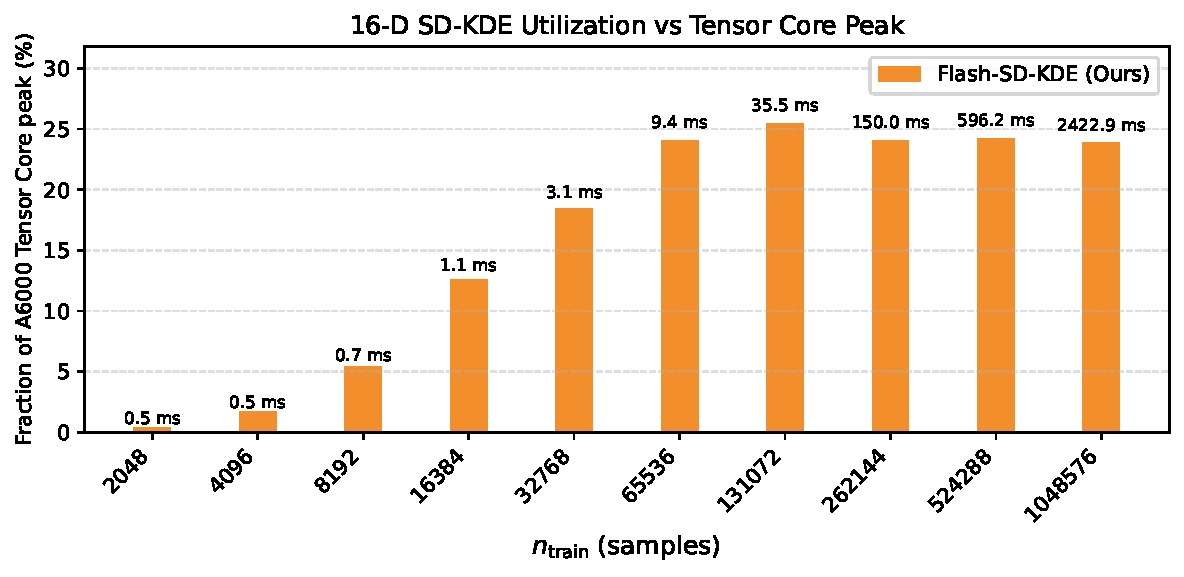
\includegraphics[width=0.9\textwidth]{figures/util_16d_sdkde_tensorcore.pdf}
  \caption{Utilization (percentage of RTX A6000 Tensor Core peak) for the 16-D
           SD-KDE pipeline, computed via the flop model from
           Section~\ref{sec:method}; bars are annotated with the observed
           runtimes (ms).}
  \label{fig:triton_sd_kde_nd_util}
\end{figure*}
% [MOVED TO Appendix~\ref{app:kernel_tuning}: The exact launch-parameter grid is reproducibility detail.  We keep the selected best configuration and effect size in the main text and move the full sweep description to Appendix~\ref{app:kernel_tuning}.]
\begin{comment}
Nsight Systems traces show that roughly $95\%$ of the SD-KDE runtime at
$n_{\text{train}}=32\text{k}$, $n_{\text{test}}=4\text{k}$ is spent computing
the empirical score.  We therefore concentrated optimization effort on the
score kernel, sweeping the launch parameters to raise utilization.  Specifically
we varied:
\begin{itemize}
  \item $BLOCK\_M \in \{32, 64, 128, 256\}$,
  \item $BLOCK\_N \in \{32, 64, 128, 256, 512, 1024\}$,
  \item $num\_warps \in \{1, 2, 4, 8\}$,
  \item $num\_stages \in \{1, 2, 4\}$,
\end{itemize}
and selected the combination that minimized runtime.  For this workload we
found that $BLOCK\_M=64$, $BLOCK\_N=1024$, $num\_warps=2$, and $num\_stages=2$
gave the best overall performance, increasing measured FLOP utilization by
more than $2\times$ relative to smaller-tile settings.
\end{comment}
% [END MOVED TO Appendix~\ref{app:kernel_tuning}]

% \begin{revadded}
Nsight Systems traces show that roughly $95\%$ of the SD-KDE runtime at $n_{\text{train}}=32\text{k}$, $n_{\text{test}}=4\text{k}$ is spent computing the empirical score.  We therefore tune the score-kernel launch configuration; the full grid is given in Appendix~\ref{app:kernel_tuning}.  The best setting uses $BLOCK\_M=64$, $BLOCK\_N=1024$, $num\_warps=2$, and $num\_stages=2$, increasing measured FLOP utilization by more than $2\times$ relative to smaller-tile settings.
% \end{revadded}

Beyond the launch-parameter sweep, two design choices account for most of the
speedup over a standard tiling implementation:
\begin{enumerate}
  \item \textbf{Tensor-Core tiling:} all high-dimensional dot products are
        processed as $16 \times 16$ tiles with Tensor Core
        acceleration, allowing the GEMM portion of the score and KDE kernels
        to run near the TF32 roofline.
  \item \textbf{Streaming accumulation:} we never materialize full
        $n_{\text{train}}\times n_{\text{train}}$ (or query) matrices; instead
        we stream tiles through registers and rely on atomic reductions to keep
        global-memory traffic linear in $n$.
\end{enumerate}

Appendices~\ref{app:streaming_ablation} and~\ref{app:tc_ablation} quantify the
factors.  At $n_{\text{train}}=65{,}536$ and
$n_{\text{test}}=8{,}192$, streaming reduces peak extra GPU allocation from
$\sim\!16$ GB to $\sim\!16$ MB and gives a $55.7\times$ speedup over
full materialization.  Holding the streamed implementation fixed, enabling
Tensor-Core tiling gives a $4.94\times$ speedup at
$n_{\text{train}}=32{,}768$ and remains near $5\times$ at the largest
sizes.  Thus streaming makes the exact quadratic computation fit in memory,
while Tensor Cores supply the large-$n$ throughput.

Together these optimizations push the kernels close to the hardware limit.
Nsight Compute's ``Speed of Light'' report shows $\sim 68\%$ SM throughput and
roughly $90\%$ L1 throughput for the score kernel at
$n_{\text{train}}=32\text{k}$ and $n_{\text{test}}=4\text{k}$, which is
consistent with the tensor-core utilization trends in
Figure~\ref{fig:triton_sd_kde_nd_util}: we cannot reach the nominal Tensor
Core peak because the kernel still executes substantial non-Tensor-Core work
(norms, exponentials, atomics).  At these utilization levels we stopped
further low-level tuning, since additional optimizations would likely yield
only modest incremental gains.










